\subsection{Introduction}
	This section is divided in two parts, the first one describe the implementation of the algorithm in a laptop computer. The objective is to get a reference to compare the results of the final implementation. The second one is a description of the final application and its results.
	During this experiments, five datasets were used. These datasets were provided by the GRVC, captured in the testbed of CATEC \cite{CATEC}, and were used previously by a partner. These datasets, composed by a number of images and data provided by a VICON system (Time, position and orientation of quadrotors), and Representing different situations, yielded a number of interesting results that will be gathered at the end of this chapter. 

	Figure: \ref{fig:frames_PC} shows an example of captured image from the camera and the result of the segmentation algorithm. Particularly, we were looking for orange color (The cap of the quadrotor in this case). However unlike simulation, where there was only one object as the result of segmentation, the algorithm return many targets. The first sift is by size, we do not consider tiny objects that use to be noise and are quantitative smaller than the target.
		
	\begin{figure}[h]
		\centering
		\begin{subfigure}{0.49\linewidth}
			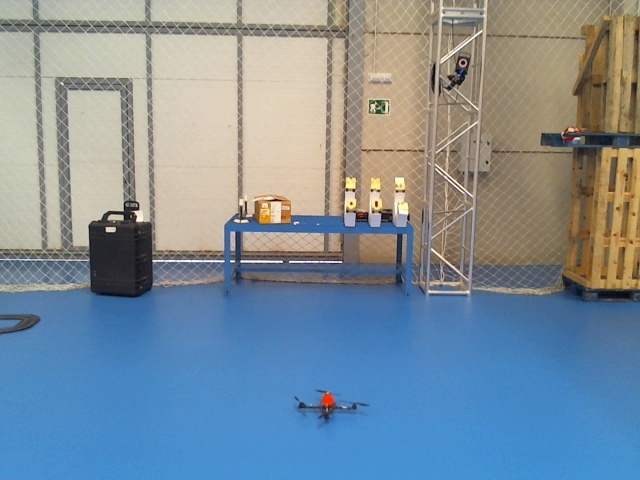
\includegraphics[width=\linewidth]{../Images/c4/image_ori}
			\caption{Original Image}
			\label{fig:image_ori}
		\end{subfigure}
		%--------------------------------------------------------------------
		\begin{subfigure}{0.49\linewidth}
			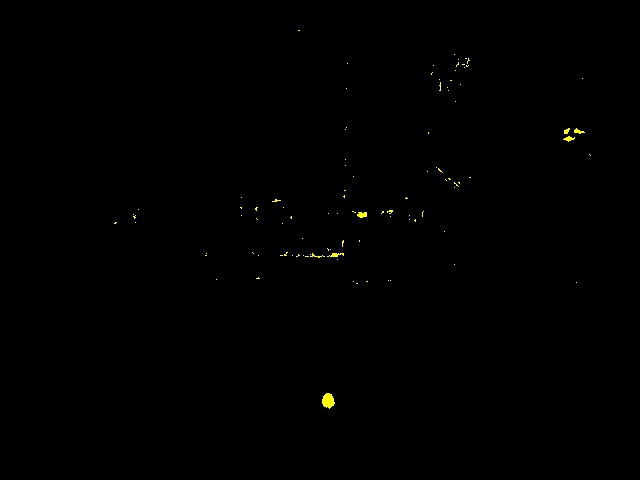
\includegraphics[width=\linewidth]{../Images/c4/image_seg}
			\caption{Segmented Image}
			\label{fig:image_seg}
		\end{subfigure}
		\caption{Images to and from algorithm}
		\label{fig:frames_PC}
	\end{figure}	


	Following sections shows the results of the described algorithm while running completely on the same computer and afterwards using the definitely structure of the system (Ground Station on PC and the capture and segmentation on the onboard computer) with the provided datasets.

\subsection{Complete Test in PC}
	In this situation, the algorithm runs in a Desktop computer using a USB camera. Summarizing:
	
	\begin{itemize}
		\item{Camera: 30 Hz and pictures of 640x480 (Logitech c525)}
		\item{Intel core i7 2.20 GHz. Usage 7\%}
		\item{6 GB of RAM. Usage $\sim$ 5000 KB}
	\end{itemize}
		
	\subsubsection{Ground Tracking algorithm}
	
	Here segmentation runs at $\sim$ 58 FPS  \ref{fig:fps_PC}. etc... etc....
	
	
	\begin{figure}[ht]
		\centering
		\begin{subfigure}[ht]{0.45\linewidth}
			\centering
				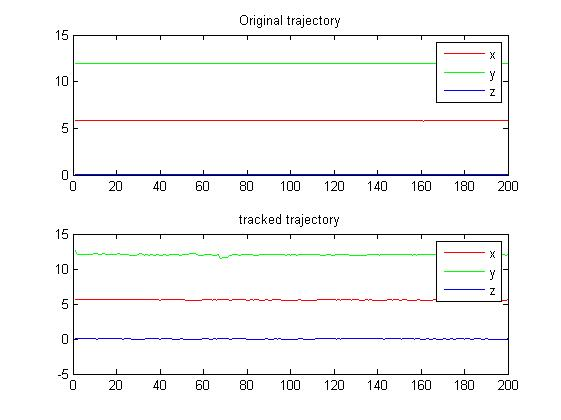
\includegraphics[width=\linewidth]{../Images/c4/trajs}
				\caption{Original and tracked trajectories}
				\label{fig:trajectories_PC}
		\end{subfigure}
		~
		\begin{subfigure}[ht]{0.45\linewidth}
			\centering
			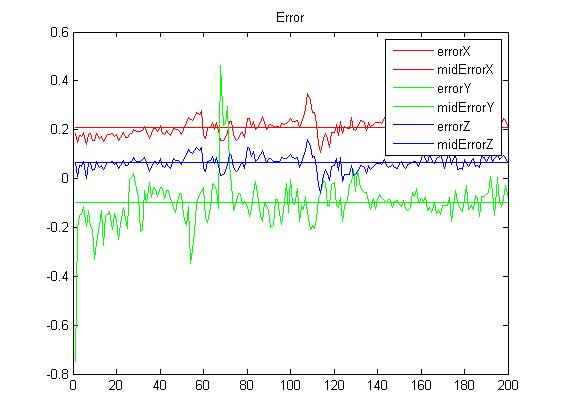
\includegraphics[width=\linewidth]{../Images/c4/errors}
			\caption{Error between real and tracked trajectories}
			\label{fig:errors_PC}
		\end{subfigure}
	\end{figure}
			
	%\begin{figure}[ht]
	%	\centering
	%	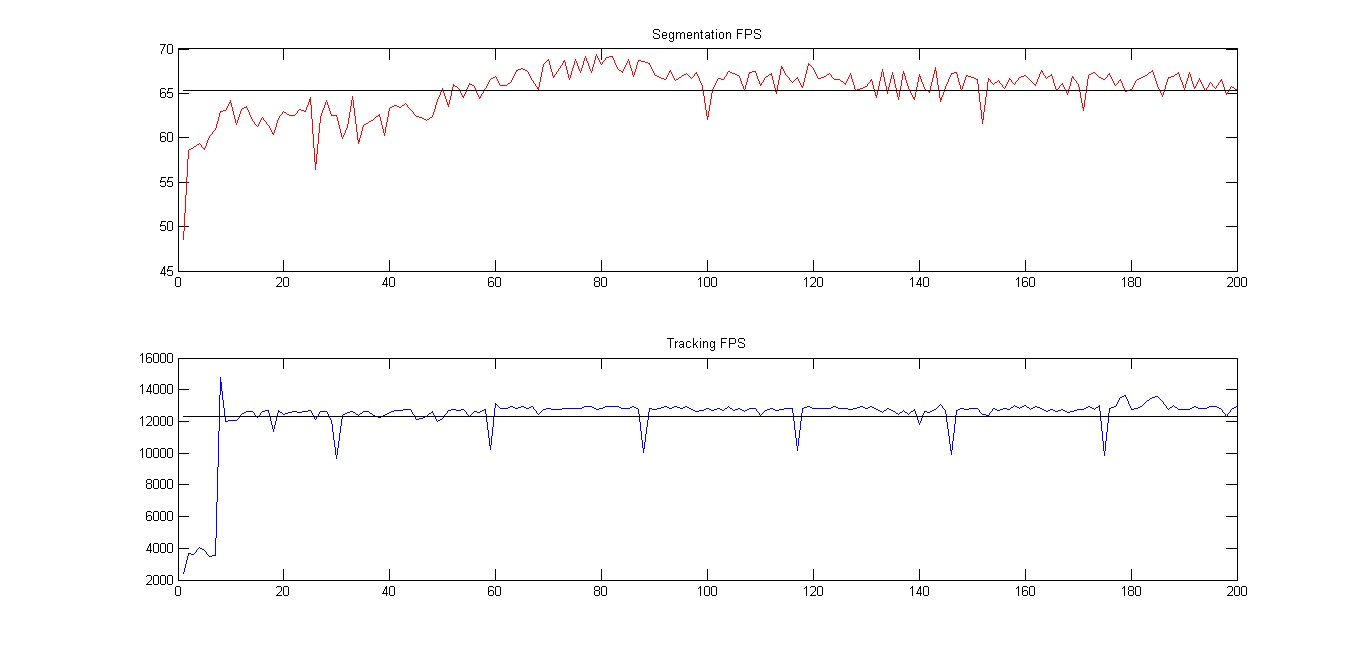
\includegraphics[width=\linewidth]{../Images/c4/fps}
	%	\caption{}
	%	\label{fig:fps_PC}
	%\end{figure}
		
	\subsubsection{Stereo Tracking algorithm}
	Here segmentation runs at $\sim$ 54 FPS  \ref{fig:fps_PC}. etc... etc....
	
	\begin{figure}[ht]
		\centering
		\begin{subfigure}[ht]{0.45\linewidth}
			\centering
				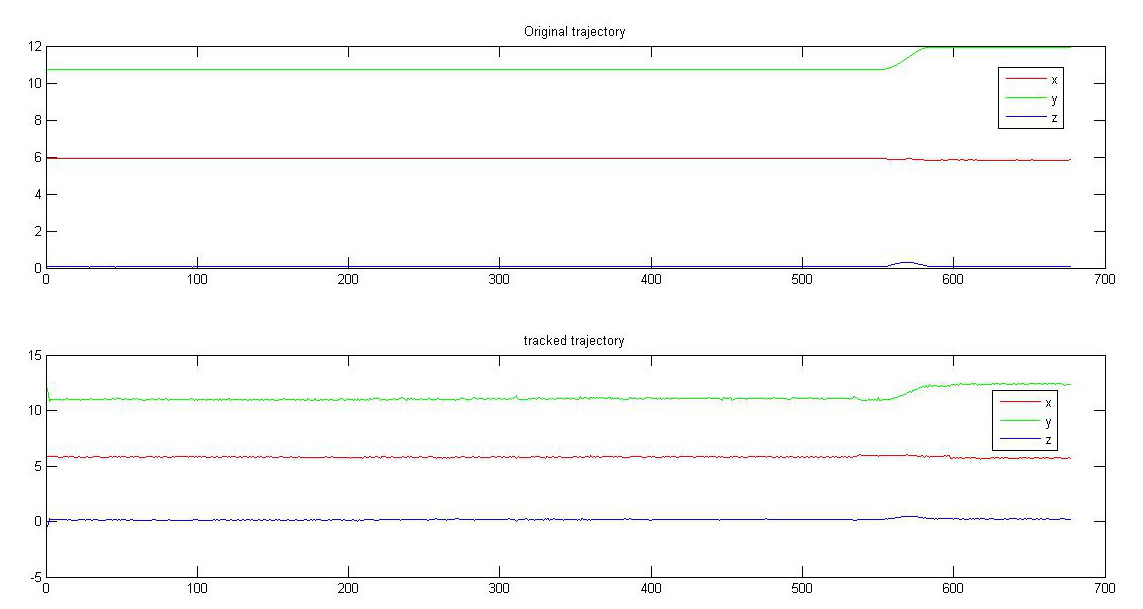
\includegraphics[width=\linewidth]{../Images/c4/trajs_stereo}
				\caption{Original and tracked trajectories}
				\label{fig:trajectories_stereo_PC}
		\end{subfigure}
		~
		\begin{subfigure}[ht]{0.45\linewidth}
			\centering
			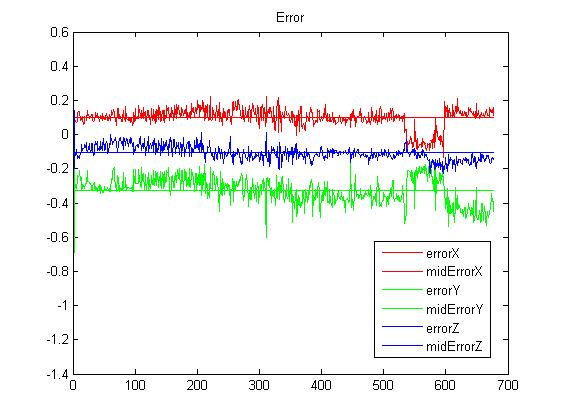
\includegraphics[width=\linewidth]{../Images/c4/errors_stereo}
			\caption{Error between real and tracked trajectories}
			\label{fig:errors_stereo_PC}
		\end{subfigure}	
	\end{figure}

	
\subsection{Test with Odroid and Ground Station}

	\subsubsection{Ground Tracking algorithm}
	
	\subsubsection{Stereo Tracking algorithm}